\subsection{SURF orientering}
SURF gør brug af Haar-wavelet filtre, når en orientering for interessepunkter skal bestemmes, og i deskriptoren. Haar-wavelet er et boksfilter, med størrelse ($N\times N$), hvor halvdelen af alle indgangene er 1 og den anden halvdel er -1. Filtret i figur \ref{fig:haarwavelet} kaldes $dx$ (venstre) og $dy$ (højre).
Når der i dette afsnit refereres til $\sigma$, skal dette forstås som sigmaværdien, der svarer til den anvendte filterstørrelse. Den kan udregnes ved:
\begin{equation}
\sigma = \dfrac{0.4\cdot\text{filterstørrelse}}{3}
\end{equation}
\begin{figure}[H]
    \centering
    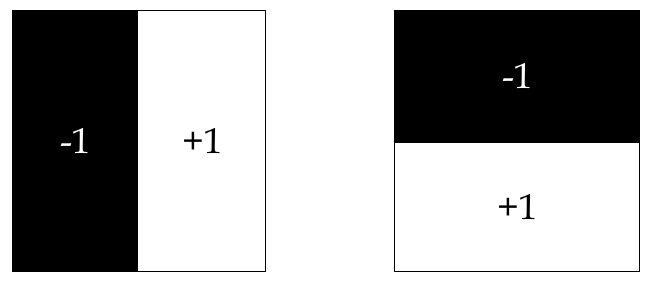
\includegraphics[width=0.55\textwidth]{fig/haarwavelet.png}
     \vspace{-1em}
    \begin{center}    
       \caption{\footnotesize \textit{{Haar-wavelet filter. venstre kaldes $d_x$ og højre $d_y$.}}}
    \label{fig:haarwavelet}
     \end{center}
     \vspace{-2.5em}
  \end{figure} \noindent
$dx$ og $dy$ foldes med punkter der ligger i et cirkulært område omkring interessepunktet. Disse to dataindsamlingsvinduer $D_x$ og $D_y$, med radius $6\sigma$, har en afstand mellem punkterne, på $\sigma$. $D_x$ og $D_y$ foldes med en Gausskerne, hvor $\sigma_{Gauss} = 2.5\sigma$.
\begin{figure}[H]
    \centering
    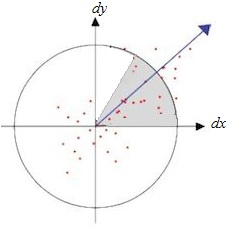
\includegraphics[width=0.3\textwidth]{fig/surforientation.jpg}
     \vspace{-1em}
    \begin{center}    
       \caption{{\footnotesize \textit{Hver punkt svarer til en vektor. Dataindsamlingsvinduet(gråt) på $60^{\circ}$, summerer vektorer, der ligger indenfor $0^{\circ}-60^{\circ}$, $60^{\circ}-120^{\circ}$,..., $300^{\circ}-360^{\circ}$. Den af de summerede vektorer der er længst, udgør punktets retning}}}
    \label{fig:surforientation}
     \end{center}
     \vspace{-2.5em}
  \end{figure} \noindent
$D_x$ og $D_y$ udgør et sæt af punkter, der kan opstilles som illustreret i figur \ref{fig:surforientation}. Hvert punkt udgør en vektor. Et vindue på $60^{\circ}$, summerer alle vektorene, der ligger indenfor dets rækkevidde (grå markering). Af de summerede vektorer, udgør den længste vektor, punktets orientering. Dette er illustreret i figur \ref{fig:surforientation}. Der er her taget en beslutning om, at vinduet udregner summen af vektorer, indenfor seks positioner ($0^{\circ}-60^{\circ}$, $60^{\circ}-120^{\circ}$,..., $300^{\circ}-360^{\circ}$).
\\
Ovenstående udregning, tildeler alle interessepunkter en orientering $\theta$.
\subsubsection*{Algoritme: SURF Orientering}
\begin{tabbing}
Input\quad \= : \= Billede $I$\\
$\text{ }$ \> : \>  Interessepunkter $p \in (x, y)$ \\
Output \text{ } \> : \> Interessepunkter med orientering $p \in (x, y, \theta)$
\end{tabbing}
\begin{enumerate}
\item Orienteringen af interessepunktet findes, ved at beregne $D_x$, $D_y$ i et cirkulært område, med radius $6\sigma$, og afstand $\sigma$, mellem punkterne. 
\item $D_x$, $D_y$ foldes med en Gausskerne, med $\sigma_{Gauss} = 2.5\sigma $.
\item Den, af de summerede vektorer, der ligger indenfor $60^{\circ}$, bruges til at tildele orientering $\theta$ til interessepunktet.
\end{enumerate}